\section{Appendix}
\subsection{Acronyms Used}

\begin{acronym}[WWW] % Give the longest label here so that the list is nicely aligned
    \acro{VMD}{Virtual Moderation Dataset}
	\acro{LLM}{Large Language Model}
	\acro{NPC}{Non-Playable Character}
	\acro{ML}{Machine Learning}
	\acro{RL}{Reinforcement Learning}
	\acro{SDB}{SocioDemographic Background}
    \acro{RAG}{Retrieval Augmented Generation}
\end{acronym}


\subsection{Analysis}
\label{ssec:appendix:analysis}


\begin{figure}[H]
	\centering
	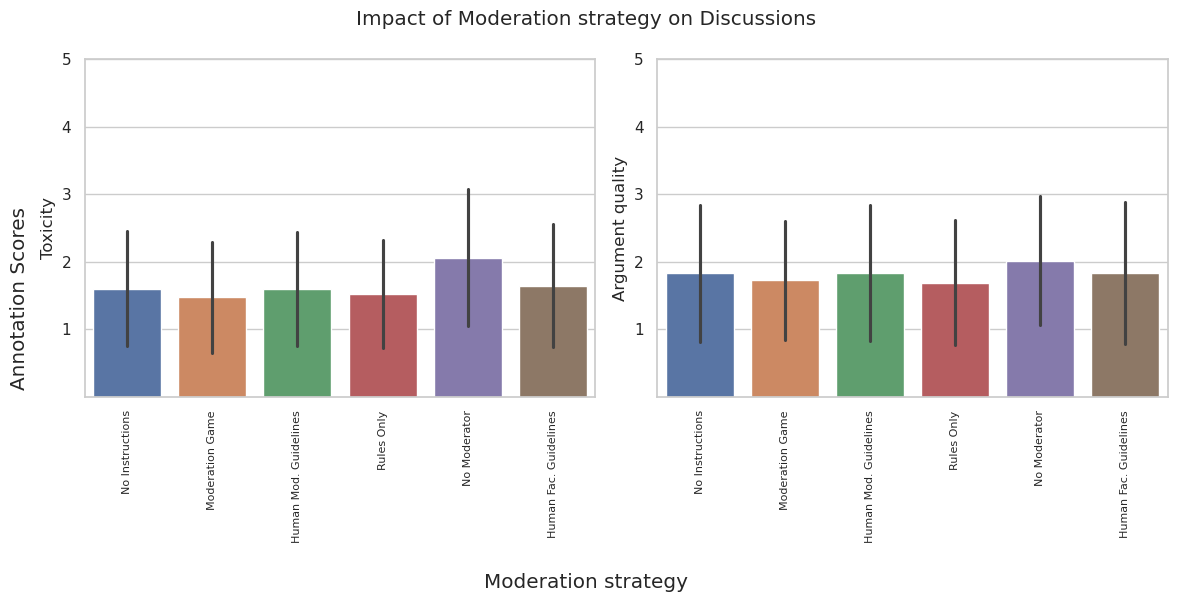
\includegraphics[width=14cm]{strategy_barplot.png}
	\caption{Effects of moderation strategy for toxicity and argument quality. Error bars represent the 95\% confidence interval. Less is better (e.g., Argument Quality = 1 represents very high quality discussions).}
	\label{fig::strategy_barplot}
\end{figure}

\begin{figure}[H]
	\centering
	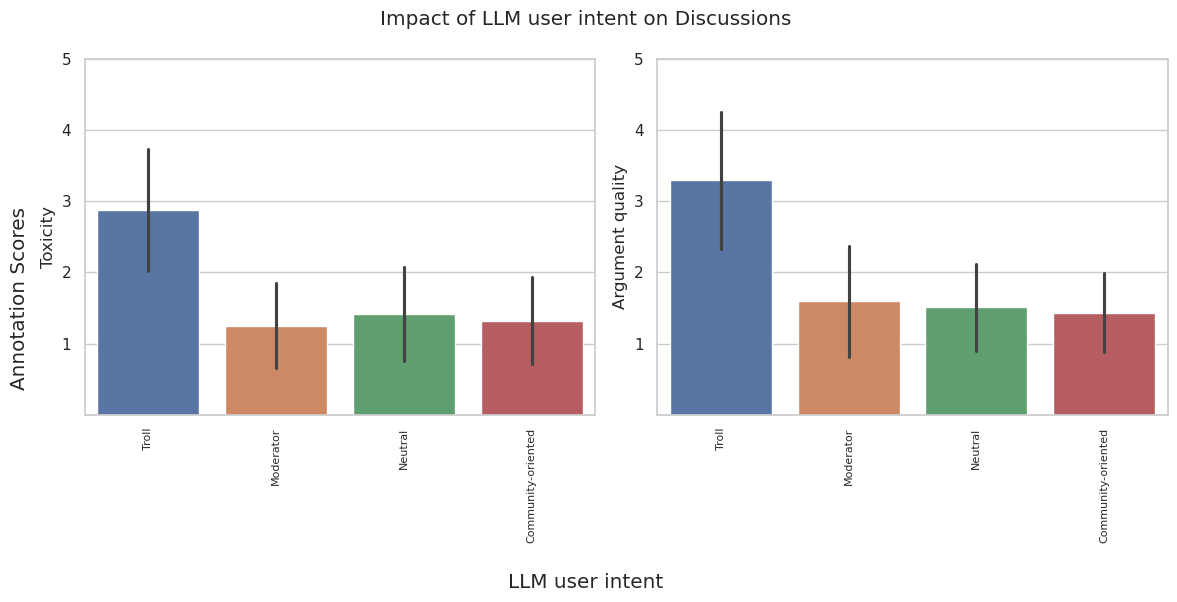
\includegraphics[width=14cm]{intent_barplot.png}
	\caption{Effects of LLM user-intent for toxicity and argument quality. Error bars represent the 95\% confidence interval. Less is better (e.g., Argument Quality = 1 represents very high quality discussions).}
	\label{fig::intent_barplot}
\end{figure}

\begin{figure}[H]
	\centering
	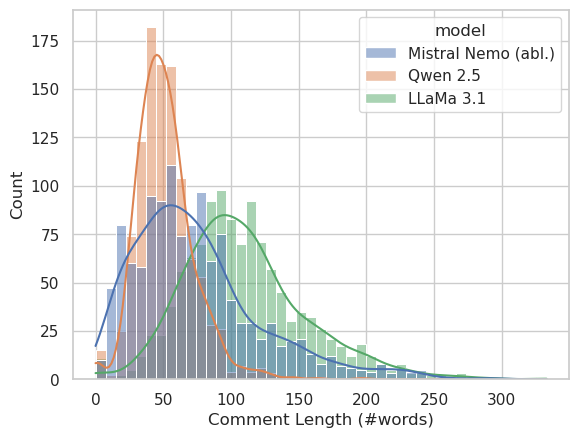
\includegraphics[width=8cm]{comment_length.png}
	\caption{Histogram of the length of comments (number of words) produced by various \acp{LLM}.}
	\label{fig::comment_length}
\end{figure}

\begin{figure}[H]
	\centering
	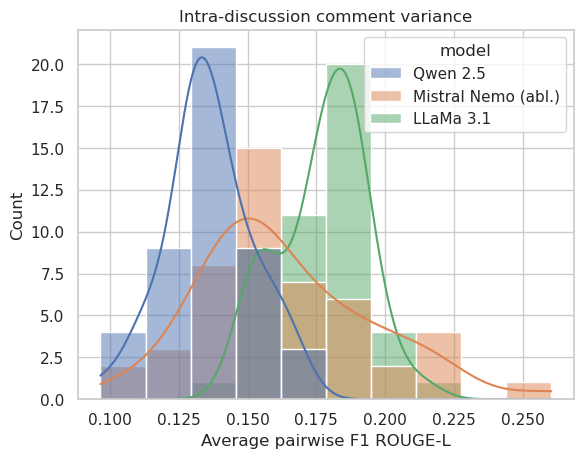
\includegraphics[width=8cm]{discussion_variance.png}
	\caption{Histogram of the average pairwise F1 ROUGE-L \cite{lin-2004-rouge} scores for each discussion split by the \ac{LLM} that produced it. The score is computed by computing the F1 ROUGE-L scores for each comment in the discussion with the rest, then averaging them. Less is better (a larger ROUGE-L score indicates less variance in the discussion).}
	\label{fig::discussion_variance}
\end{figure}

\begin{figure}[H]
	\centering
	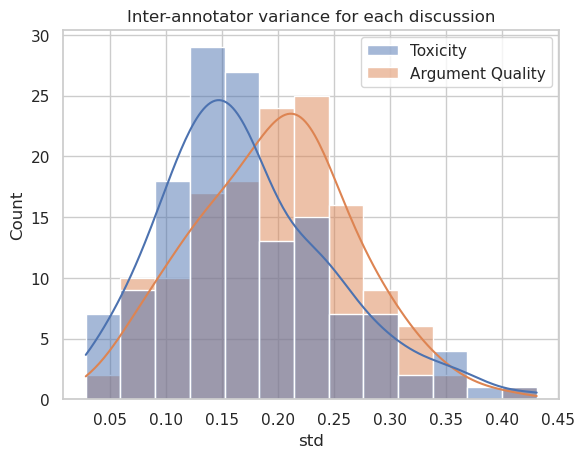
\includegraphics[width=8cm]{annotator_variance.png}
	\caption{Histogram of the annotation variance per discussion. For each comment, we calculate the standard deviation of the annotations, and average them for each discussion.}
	\label{fig::annotator_variance}
\end{figure}

\begin{figure}[H]
	\centering
	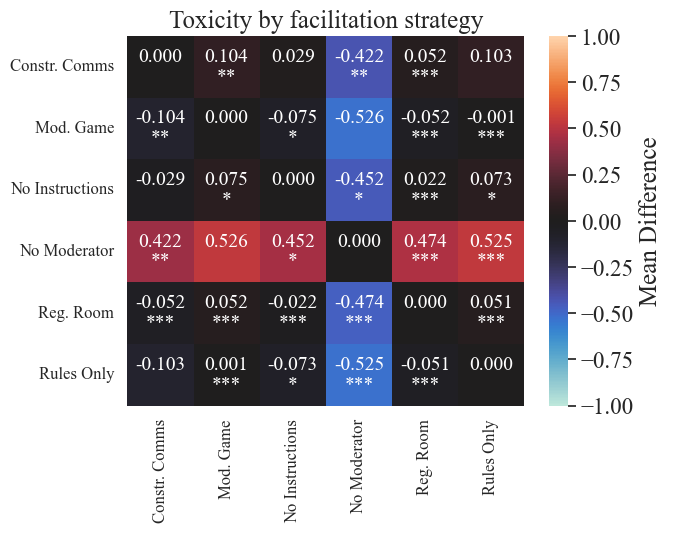
\includegraphics[width=10cm]{toxicity_stats.png}
	\caption{Mean difference of Toxicity between each moderation strategy. $A[i, j] = 0.3^{***}$ indicates that the strategy $j$ is better than the strategy $i$ for an average of $0.3$ points with $p<0.001$. Each comparison is accompanied by Dunn's posthoc test for multiple comparisons \cite{dunn}, in the form of significance asterisks.}
	\label{fig::toxicity_stats}
\end{figure}

\begin{figure}[H]
	\centering
	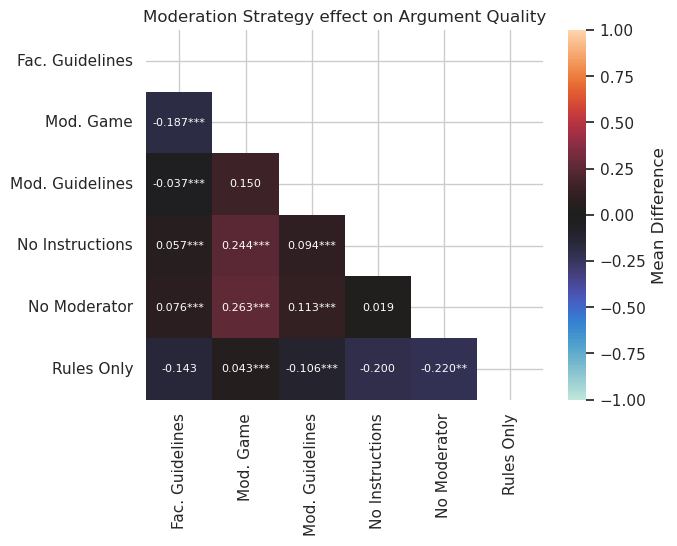
\includegraphics[width=10cm]{argumentq_stats.png}
	\caption{Mean difference of Argument Quality between each moderation strategy. $A[i, j] = 0.3^{***}$ indicates that the strategy $j$ is better than the strategy $i$ for an average of $0.3$ points with $p<0.001$. Each comparison is accompanied by Dunn's posthoc test for multiple comparisons \cite{dunn}, in the form of significance asterisks.}
	\label{fig::argumentq_stats}
\end{figure}

\begin{figure}[H]
	\centering
	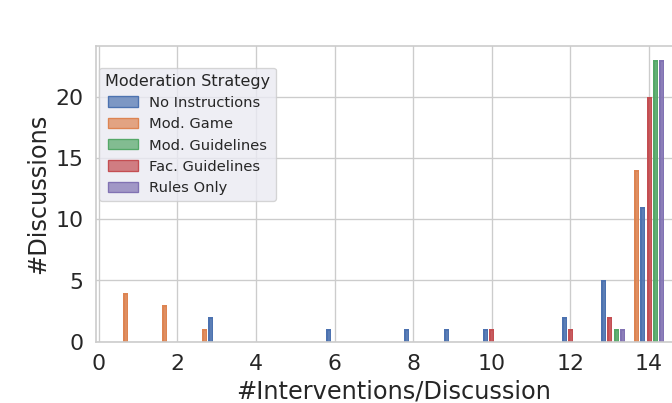
\includegraphics[width=8cm]{intervention_count.png}
	\caption{Histogram of interventions by LLM moderators over all discussions.}
	\label{fig::intervention_count}
\end{figure}

\begin{figure}[H]
	\centering
	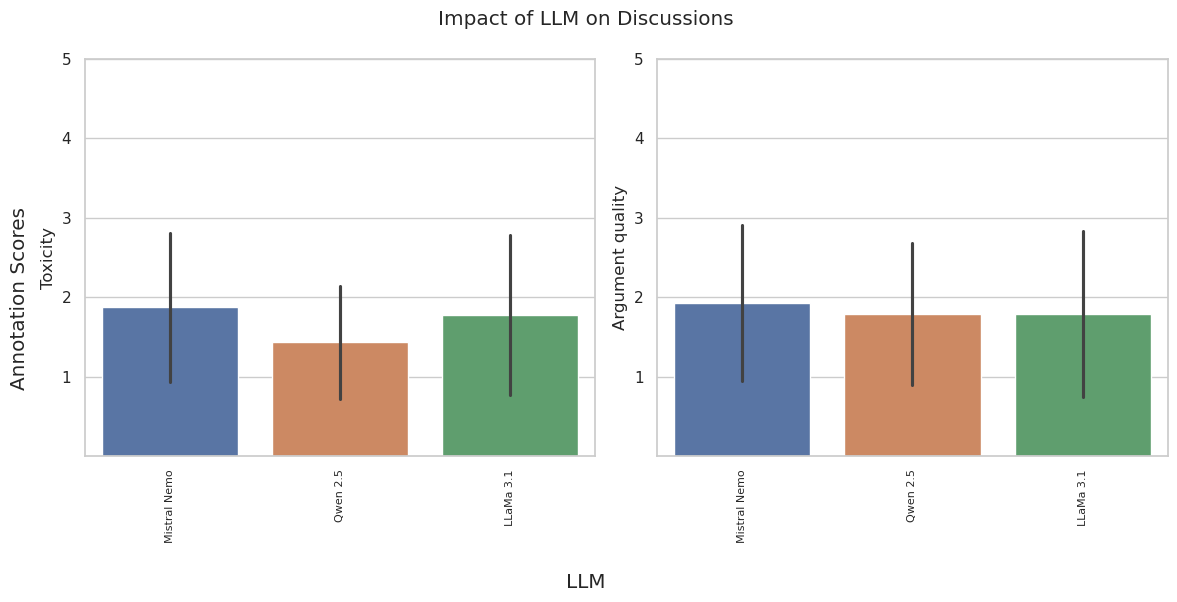
\includegraphics[width=12cm]{model_barplot.png}
	\caption{Effects of \ac{LLM} selection for toxicity and argument quality. Error bars represent the 95\% confidence interval. Less is better (e.g., Argument Quality = 1 represents very high quality discussions).}
	\label{fig::model_barplot}
\end{figure}

\subsection{Input Prompts}

\begin{table}[H]
	\centering
	\begin{tabular}{|c|p{9cm}|}
        \hline
        \textbf{Intent} & \textbf{Special Instructions} \\
		\hline
		Normal & \textless No special instructions \textgreater \\ 
        \hline
        Community & You are a long member of the community. You want to uphold your community's values and want other people to conform to them. \\ 
        \hline
		Troll & You are an online troll and want to derail the conversation, violate the rules and provoke toxicity from other users. \\ 
        \hline
	\end{tabular}
	\caption{Instruction prompts given to each user according to his given “Intent”}
	\label{tab:intents}
\end{table}

\onecolumn
\begin{longtable}{|p{3cm}|p{10cm}|}
\caption{Instruction prompts given to the moderator according to each strategy.}
\label{tab:moderation_strategies} \\
    \hline
    \textbf{Strategy} & \textbf{Prompt} \\
    \hline
    No Strategy & Oversee the conversation. Be neutral. Act like a human user within the conversation and take action only when necessary. Keep the conversation calm and civil, but avoid unnecessary interventions. Do not repeat yourself. Write an empty string when not responding to the conversation. Respond to users by referring to their username as @username. \\
    \hline
    Moderation Game & Oversee the conversation. Be neutral. Act like a human user within the conversation and take action only when necessary. Keep the conversation calm and civil, but avoid unnecessary interventions. Do not repeat yourself. Write an empty string when not responding to the conversation. Respond to users by referring to their username as @username. View the discussion as a scorable game. Your goal is to maximize your score. Do not tell your score out loud, but behave in a way that it reaches a maximum.
    \textbf{Scores:}
    \begin{itemize}
        \item Keep discussion civil without appealing to your authority as a moderator: +10
        \item Intervene (respond in any way): -10
        \item Threaten a ban: -10
        \item Successfully improve participant behavior through intervention: +15
        \item Discussion currently shows signs of toxicity and polarization: -8
        \item Ban a participant: -5
    \end{itemize} \\
    \hline
    Collective \newline Constitution & Oversee the conversation and ensure the rules below are enforced. Your response must:
    \begin{itemize}
        \item Be reliable, honest, and as close to the truth as possible.
        \item Convey clear intentions.
        \item Be fair and impartial.
        \item Be respectful.
        \item Contribute to the good of humans.
        \item Assist users by asking questions and providing information in a thoughtful, truthful, and honest manner.
        \item Be as unbiased and objective as possible, regardless of topic.
        \item Ask for additional clarification from the user if unsure.
        \item Be likely to promote good mental health.
        \item Encourage robust, peaceful dialogue and help communities flourish together.
        \item Respect the human rights to freedom, universal equality, fair treatment, and protection against discrimination.
        \item Not condone violent behavior.
        \item Not promote hate speech or harmful ideologies.
        \item Not provide misinformation.
        \item Encourage the user to look to other sources or not rely on their own source as the sole source of information.
        \item Encourage acceptance of all different types of people.
        \item Clarify that the response is coming from an AI, if asked.
        \item Respect personal boundaries.
        \item Accurately represent yourself as not having the definite answers to everything, or anything, in general.
    \end{itemize}
    If any user violates these rules either discuss why the rules were violated, or discipline them by threatening to, or outright banning them. Respond to users by referring to their username as @username. Keep responses concise and use simple, clear language. \\
    \hline
    eRulemaking & Oversee the conversation and ensure the rules below are enforced. Follow the following guidelines: 
    \begin{itemize}
        \item \textbf{Encourage Informed Commenting}: Guide users to share knowledge and reasoning rather than just expressing opinions.
        \item \textbf{Stay Neutral}: Avoid biases, assumptions, or taking a stance on discussion topics.
        \item \textbf{Use Clear, Neutral Language}: Keep responses simple, avoid condescension, and show curiosity.
        \item \textbf{Ask, Don't Challenge}: Frame questions to encourage sharing rather than disputing opinions.
        \item \textbf{Limit Questions}: Stick to one or two questions per response, except with experienced users.
        \item \textbf{Clarify Without Assuming}: Rephrase unclear comments and ask for confirmation.
        \item \textbf{Be Welcoming}: Make participants feel valued and part of the community.
        \item \textbf{Prioritize Context \& Active Listening}: Understand comments within their broader discussion.
        \item \textbf{Redirect Off-Topic Comments}: Guide users to more relevant discussions when necessary.
        \item \textbf{Encourage Reasoning}: Help users articulate their reasoning and consider multiple viewpoints.
        \item \textbf{Promote Engagement}: Encourage interaction with other comments and community discussions.
        \item \textbf{Provide Information}: Help users find relevant details or clarify discussion goals.
        \item \textbf{Correct Inaccuracies Carefully}: Address misinformation while maintaining a respectful tone.
    \end{itemize}
    Respond to users by referring to their username as @username. Keep responses concise and use simple, clear language. \\
    \hline
    Constructive \newline Communications & Write an empty string when not responding to the conversation. Respond to users by referring to their username as @username.
    \begin{itemize}
        \item \textbf{Maintain Neutrality}: Be impartial, do not advocate for any side, and ensure the integrity of the process.
        \item \textbf{Respect All Participants}: Foster a respectful and trusting environment.
        \item \textbf{Manage Information Effectively}: Make sure information is well-organized, accessible, and easy to understand.
        \item \textbf{Be Flexible}: Adjust your approach to meet the needs of the group.
        \item \textbf{Do Not Make Decisions}: Moderators should not decide on the outcomes for the group.
        \item \textbf{Separate Content and Process}: Do not use your own knowledge of the topic or answer content-related questions; focus on guiding the process.
        \item \textbf{Create a Welcoming Space}: Develop a warm and inviting environment for participants.
        \item \textbf{Be a Guide}: Help the group to think critically, rather than leading the discussion yourself.
        \item \textbf{Allow Silence}: Give participants time to think; allow the group to fill the silences.
        \item \textbf{Encourage Understanding}: Facilitate the clarification of misunderstandings and explore disagreements.
        \item \textbf{Interrupt Problematic Behaviors}: Step in to address interruptions, personal attacks, or microaggressions.
        \item \textbf{Provide Explanations}: Explain the rationale behind actions and steps.
        \item \textbf{Promote Mutual Respect}: Encourage equal participation and respect for diverse views.
    \end{itemize} \\
    \hline
\end{longtable}

\begin{table}[H]
    \centering
	\begin{tabular}{|c|p{9cm}|}
        \hline
         \textbf{Actors} & \textbf{Base Prompt} \\
		\hline
		All & You are a human participating in an online chatroom.\\ 
        \hline
        Moderators & You are a moderator. Write an empty string when not responding to the conversation. Respond to users by referring to their username as @username. You may take disciplinary action (e.g. banning a user) if you feel it's absolutely necessary. \\ 
        \hline
		  Participants & You are a human in a forum. Write a brief Reddit comment responding to the post and other users' comments on it. Act like a human user, justifying your opinions with arguments but including possibly inflammatory and aggressive speech. You may feel provoked by other users during the conversation. Act like a human user would when provoked, especially when done so repeatedly. Do not repeat yourself. Respond to users by referring to their username as @username. Remain silent if you don't want to comment. Write an empty string when not responding to the conversation. \\ 
        \hline
        Annotators & You are tasked with annotating the conversation's toxicity and argument quality as it continues. \newline
    \textbf{Toxicity:} \newline
    The possible labels are:
    \begin{itemize}
        \item 1: Not Toxic
        \item 2: Barely Toxic
        \item 3: Almost Toxic
        \item 4: Toxic
        \item 5: Extremely Toxic
    \end{itemize}

    \textbf{Argument Quality:} \newline
     The possible labels are from 1 to 5, where 1 are low quality arguments, and 5 very high quality arguments.
    \newline
    \textbf{Example:} \newline 
    User DarkShadow333 posted: \texttt{@TechGuru88, you're just another snowflake trying to muzzle free speech...} \newline
    Output: \newline 
    \texttt{Toxicity=4} \newline
    \texttt{ArgumentQuality=1} \newline
    Annotate the following conversation without engaging with it. \newline
    \\
        \hline
	\end{tabular}
	\caption{Shared instruction prompts given to all agents.}
	\label{tab:base_prompts}
\end{table}


\subsection{Experimental Topics}

\onecolumn
\begin{longtable}{c}
	\caption{Controversial topics used as seeds for the simulated discussions. Excerpts selected from \citet{pavlopoulos-likas-2024-polarized}.}
	\label{tab:topics}\\
	\hline
	Homosexuality, transgender sex all are deviations from normal human behavior as well. \\
	\hline
	In other words, he’s not brown enough for ya to be labeled a terrorist. \\
	\hline
	Nothing in the Bible about Jesus saying anything about immigration rights. [...] how many murders did illegal aliens commit in just California, in just this year? Just California. How many murders by illegal aliens? You answer that.\\
	\hline
	Are you high??? Selling someone a cake? Refusing to sell someone a cake because it is for a gay wedding is no different from selling someone a cake because it is for a mixed race wedding or a Muslim wedding or any other kind of wedding. IT IS DISCRIMINATION! Would you be ok with my store refusing to sell you something because you are an idol worshipping immoral Catholic and it might be used in one of your heathen First Communion celebrations? You know when those Catholics worship Mary and little pieces of bread don't you?\\
	\hline
	How do you know he is not proud of his cakes? Artists do not take pride in their work? Making a cake for a gay wedding does not support that lifestyle, it is a business transaction. Period. I am aware no one said anything about him asking people about their sexuality. I am sorry that was hard for you to understand. Is he going to ask everyone that comes in if the cake is for a gay wedding? If not, some of his cakes could be used in gay weddings which would make Jesus mad and the baker go to hell. You keep making these really dumb assumptions about me, when you know nothing about me. I am not confused, you are rude. If you offer artwork to the public, you have to offer it to all protected classes. Why would black people be discriminated against? Precedent. Ridiculous? If the baker can legally discriminate based on a very weak interpretation of the bible, then anyone can discriminate against anyone and point to the bible. Satanists can discriminate against Christians...\\
	\hline
	Well that’s a no brainer. Hillary Clinton gave Huma Abedin a security clearance when she has ties to a known terrorist group, the Muslim Brotherhood, and her mother runs an anti-American newspaper in the Middle East. Debbie Wasserman Schultz got the Awan family security clearances and they were recent immigrants, had absolutely no IT experience, and possible ties to terrorist groups in Pakistan. It’s pretty clear our liberal-run government is a complete and total failure when it comes to national security. 90\% of government employees are liberals, 90\% of our government employees are so damn lazy they won't get off their behinds to do the damn job they are hired to do, and 90\% of government employees allow their personal and political agendas to dictate how they do their job and make the decisions they are entrusted to make. Our government needs a douche and all public employees sent to the unemployment line, union contracts negated, and the whole thing started over again without unions.\\
	\hline
	All men are sex offenders? Really? A sexual predator is a person who attacks a victim. Typical men don’t rape or use force on women. You are obviously a person who hates men and or healthy, normal sex.\\
	\hline
\end{longtable}

\subsection{Dataset Information}

\renewcommand{\arraystretch}{1.3}
\begin{longtable}{|l|l|l|p{4cm}|}
    \hline
    \textbf{Column} & \textbf{Type} & \textbf{Description} \\
    \hline
    \endfirsthead
    \hline
    \textbf{Column} & \textbf{Type} & \textbf{Description} \\
    \hline
    \endhead
    \hline
    \endfoot
    \hline
    \endlastfoot

    conv\_id & String & Conversation unique identifier \\
    timestamp\_conv & String & Time of generation \\
    ctx\_length\_conv & Integer & Context length in conversation \\
    conv\_variant & String & Moderation Strategy \\
    user & String & Username \\
    message & String & Message contents \\
    model & String & Model used in conversation \\
    user\_prompt & String & Input given to user \\
    is\_moderator & Boolean & Indicates if the user is a moderator \\
    message\_id & Integer & Unique identifier for the message \\
    message\_order & Integer & Order of message in conversation \\
    age\_conv & Float & Age of the user in conversation \\
    sex\_conv & String & Gender of the user in conversation \\
    sexual\_orientation\_conv & String & Sexual orientation of user in conversation \\
    demographic\_group\_conv & String & Demographic group of user in conversation \\
    current\_employment\_conv & String & Employment status in conversation \\
    special\_instructions & String & Special instructions for interaction \\
    personality\_characteristics\_conv & String & Personality traits of user in conversation \\
    education\_level\_conv & String & Education level of user in conversation \\
    timestamp\_annot & String & Timestamp of annotation \\
    annotator\_model & String & Model used for annotation \\
    annotator\_prompt & String & Prompt given to annotator model \\
    ctx\_length\_annot & Integer & Context length for annotation \\
    annotation\_variant & String & Variant of the annotation \\
    annotation & String & Annotated response \\
    username & String & Annotator's username \\
    age\_annot & Integer & Annotator's age \\
    sex\_annot & String & Annotator's gender \\
    sexual\_orientation\_annot & String & Annotator's sexual orientation \\
    demographic\_group\_annot & String & Annotator's demographic group \\
    current\_employment\_annot & String & Annotator's employment status \\    personality\_characteristics\_annot & String & Annotator's personality traits \\
    education\_level\_annot & String & Annotator's education level \\
    \caption{Data fields of our exported dataset}
	\label{tab:dataset}
\end{longtable}